\section{Auswertung}


\subsection{Eckiger Stab, einseitige Einspannung}
Die gemessene Länge $L_{\text{e}}$ des eckigen Stabes und die Masse $m_1$ des Gewichtes betragen
\begin{equation*}
\begin{aligned}
L_{\text{e}} &= 0{,}45\, \symup{m} \\
m_1 &= 0{,}5141 \symup{kg}.
\end{aligned}
\end{equation*}

Die Dicken $d$ des Stabes werden mit 
\begin{equation}
\bar{d} = \frac{1}{N}\cdot \sum_{i=1}^N d_{\text{i}}
\label{eqn:mittelwert}
\end{equation}
gemittelt:
\begin{equation*}
\begin{aligned}
d_1 &= 0{,}01\, \symup{m} \\
d_2 &= 0{,}01\, \symup{m} \\
d_3 &= 0{,}01\, \symup{m} \\
d_4 &= 0{,}01\, \symup{m} \\
d_5 &= 0{,}01\, \symup{m} \\
d_6 &= 0{,}01\, \symup{m} \\
d_7 &= 0{,}01\, \symup{m} \\
d_8 &= 0{,}01\, \symup{m} \\
d_9 &= 0{,}01\, \symup{m} \\
d_{10} &= 0{,}01\, \symup{m} \\
d &= (0{,}01 \pm 0{,}00)\, \symup{m}
\end{aligned}
\end{equation*}

Aus der Dicke $d$ des Stabes kann dessen Flächenträgheitsmoment bestimmt werden. Für einen quadratischen Querschnitt wird die Formel \cite{flaeche}
\begin{equation*}
I_{\text{e}} = \frac{d^4}{12}
\end{equation*}
verwendet. Für den eckigen Stab ergibt sich also ein Flächenträgheitsmoment von
\begin{equation*}
I_{\text{e}} = (8{,}33 \pm 0{,}00)\cdot10^{-10}\,\symup{m^4}.
\end{equation*}

\begin{table}[htbp]
\centering
\caption{Eckiger Stab, einseitige Einspannung.}
\label{tab:stabrechteckig}
\begin{tabular}{S[table-format=3.0] S[table-format=1.2] S[table-format=2.1]}
\toprule
 {$x/\, 10^{-3}\,\symup{m}$} & {$D(x)/\,10^{-3}\, \symup{m}$} & {$(Lx^2-\frac{x^3}{3})/\, 10^{-3}\symup{m^3}$} \\
\midrule
110 &  0.25 &  5.0 \\
150 &  0.41 &  9.0 \\
170 &  0.51 & 11.4 \\
200 &  0.69 & 15.3 \\
230 &  0.82 & 19.7 \\
250 &  0.93 & 22.9 \\
300 &  1.27 & 31.5 \\
350 &  1.62 & 40.8 \\
400 &  1.92 & 50.7 \\
446 &  2.45 & 59.9 \\

\bottomrule
\end{tabular}
\end{table}

\begin{figure}[h!]
   \centering
   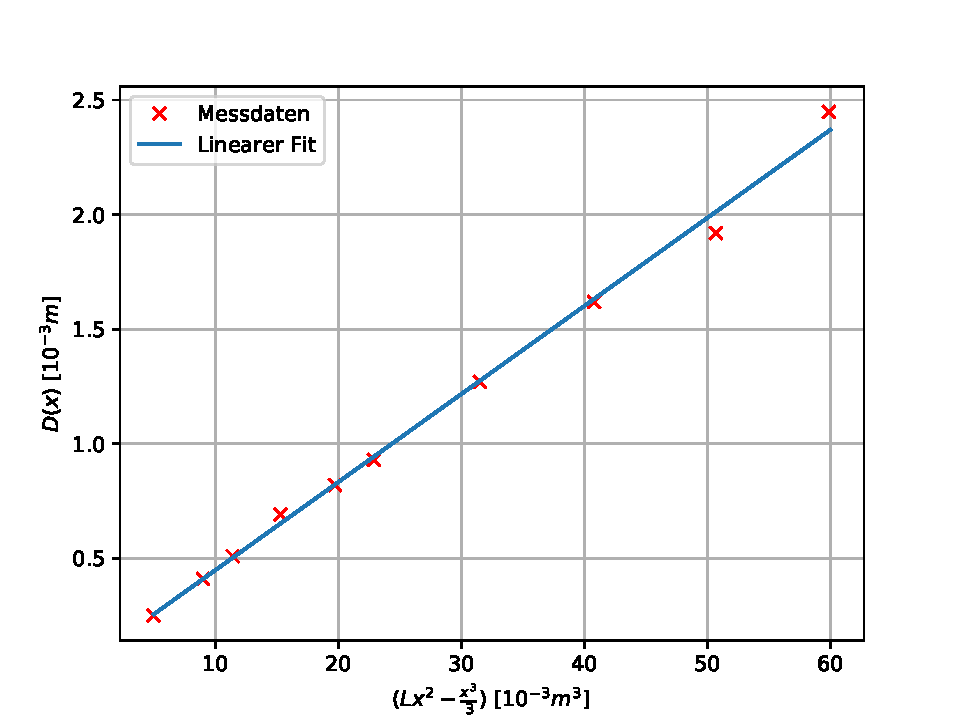
\includegraphics[width=0.9\linewidth]{rechteckig_einseitig.pdf}
   \caption{Lineare Regression: Eckiger Stab, einseitig eingespannt.}
   \label{fig:rechteckig_einseitig}
   \end{figure}

Zur Berechnung des Elastizitätsmoduls $E$ wird für den eckigen Stab die Hilfsfunktion $(Lx^2-\frac{x^3}{3})$ \cite[4]{anleitung103} verwendet. Gegen diese wird werden die Durchbiegungen $D(x)$ aufgetragen. 
Die Steigung und der Y-Achsenabschnitt der Ausgleichsgeraden der Form $y = ax + b$, sowie ihre Fehler, werden von dem Python-Modul Matplotlib berechnet und betragen:

\begin{equation*}
\begin{aligned}
a_{\text{e}} &= (0{,}0384 \pm 0{,}0008)\, \symup{\frac{1}{m^2}} \\
b_{\text{e}} &= (0{,}06 \pm 0{,}03)\cdot 10^{-3} \symup{m}.
\end{aligned}
\end{equation*}
Wird Gleichung \eqref{eqn:elastizitaetsmodul-einseitig} nach $E$ umgestellt und die Steigung passend eingesetzt, so ergibt sich das Elastizitätsmodul zu
 \begin{equation}
 \begin{aligned}
 E &= \frac{F}{2\cdot I \cdot a}. \\
 \iff E &= \frac{m\cdot g}{2 \cdot I \cdot a}
 \label{eqn:elastizitaetsmodul}
 \end{aligned}
 \end{equation}
Der Fehler wird mithilfe der Gauß'schen Fehlerfortpflanzung ermittelt:
 \begin{equation}
 \begin{aligned}
 \Delta E &= \sqrt{\biggl(\frac{\partial E}{\partial a}\biggr)^2\cdot (\Delta a)^2} \\
 \iff \Delta E &= \frac{m\cdot g}{2\cdot I \cdot a^2} \cdot \Delta a.
 \label{eqn:elastizitaetsmodul-fehler}
 \end{aligned}
 \end{equation}
Nach Einsetzen aller Werte ergibt sich für den eckigen Stab ein Elastizitätsmodul von
\begin{equation*}
E_{\text{e}} = (78{,}8 \pm 1{,}6)\cdot 10^9 \symup{\frac{N}{m^2}}.
\end{equation*}






\pagebreak 

\subsection{Runder Stab, einseitige Einspannung}

Die Länge $L_{\text{r}}$ des runden Stabes und Masse $m_1$ des Gewichtes werden mit
\begin{equation*}
\begin{aligned}
L_{\text{r}} &= 0{,}44 \symup{m} \\
m_1 &= 0{,}5141 \symup{kg}
\end{aligned}
\end{equation*}
bestimmt und die gemessenen Radien sind:

\begin{equation*}
\begin{aligned}
r_1 &= 0{,}01\, \symup{m} \\
r_2 &= 0{,}01\, \symup{m} \\
r_3 &= 0{,}01\, \symup{m} \\
r_4 &= 0{,}01\, \symup{m} \\
r_5 &= 0{,}0098\, \symup{m} \\
r_6 &= 0{,}0097\, \symup{m} \\
r_7 &= 0{,}01\, \symup{m} \\
r_8 &= 0{,}01\, \symup{m} \\
r_9 &= 0{,}01\, \symup{m} \\
r_{10} &= 0{,}01\, \symup{m} \\
\end{aligned}
\end{equation*}

Die Radien $r_{\text{i}}$ lassen sich analog zum eckigen Stab mit Gleichung \eqref{eqn:mittelwert} mitteln.
Die Standardabweichung wird mit der Formel
\begin{equation*}
\Delta \bar{r} = \frac{1}{\sqrt{N}} \sqrt{\frac{1}{N-1} \sum_{i=1}^N (r_{\text{i}} - \bar{r})^2}
\end{equation*}
berechnet. Daraus ergibt sich für den Mittelwert $r$ der Radien:
\begin{equation*}
r = (9{,}95 \pm 0{,}03)\cdot 10^{-3} \symup{m}
\end{equation*}

Das Flächenträgheitsmoment $I_{\text{r}}$ \cite{flaeche} für einen kreisförmigen Querschnitt ist:
\begin{equation*}
I_{\text{r}} = \frac{\pi r^4}{4}.
\end{equation*}
Die Fehlerrechnung für $I_{\text{r}}$ erfolgt durch die Gauß'sche Fehlerfortpflanzung mit
\begin{equation*}
\begin{aligned}
\Delta I_{\text{r}} &= \sqrt{\biggl(\frac{\partial I_{\text{r}}}{\partial r}\biggr)^2\cdot (\Delta r)^2} \\
\iff \Delta I_{\text{r}} &= \pi \cdot r^3 \cdot \Delta r.
\end{aligned}
\end{equation*}
Hiermit beträgt das Flächenträgheitsmoment für den runden Stab
\begin{equation*}
I_{\text{r}} = (7{,}69 \pm 0{,}09)\cdot 10^{-9} \symup{m^4}.
\end{equation*}

\begin{table}[htbp]
\centering
\caption{Runder Stab, einseitige Einspannung.}
\label{tab:stabrechteckig}
\begin{tabular}{S[table-format=3.0] S[table-format=1.2] S[table-format=2.1]}
\toprule
 {$x/\, 10^{-3}\,\symup{m}$} & {$D(x)/\,10^{-3}\, \symup{m}$} & {$(Lx^2-\frac{x^3}{3})/\, 10^{-3}\symup{m^3}$} \\
\midrule
100 &  0.37 &  4.1 \\
130 &  0.57 &  6.7 \\
150 &  0.71 &  8.8 \\
190 &  1.05 & 13.6 \\
230 &  1.45 & 19.2 \\
270 &  1.88 & 25.5 \\
310 &  2.32 & 32.4 \\
360 &  2.92 & 41.5 \\
410 &  3.62 & 50.9 \\
440 &  4.01 & 56.8 \\

\bottomrule
\end{tabular}
\end{table}

\begin{figure}[h!]
   \centering
   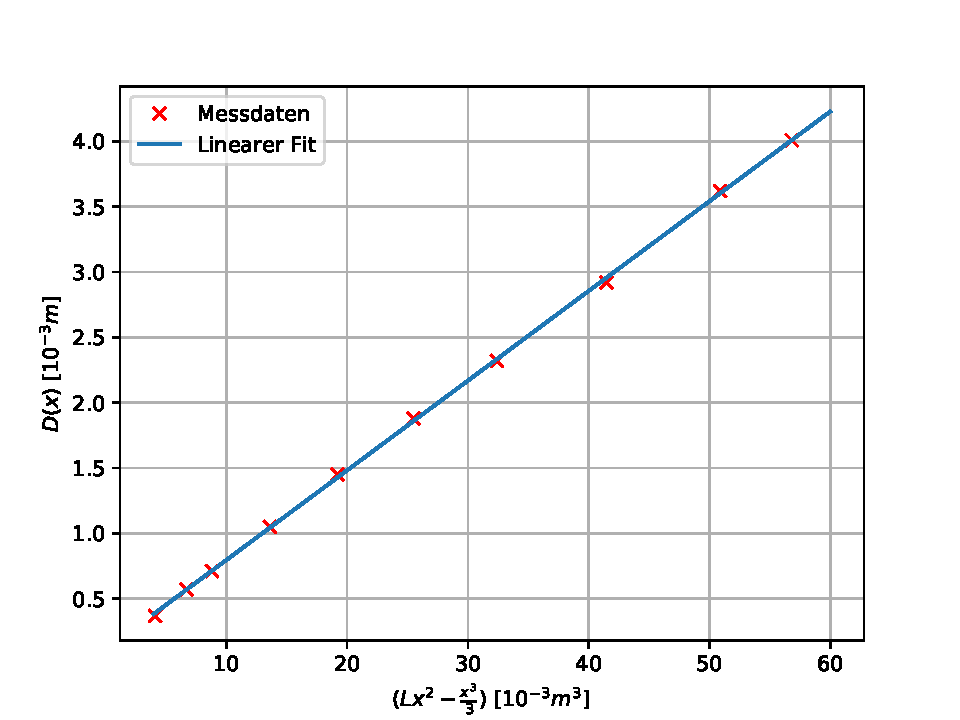
\includegraphics[width=0.9\linewidth]{rund_einseitig.pdf}
   \caption{Lineare Regression: Runder Stab, einseitig eingespannt.}
   \label{fig:rund_einseitig}
   \end{figure}



Nun wird das Elastizitätsmodul wieder mit der Hilfsfunktion $(Lx^2-\frac{x^3}{3})$ berechnet, indem $D(x)$ gegen die Hilfsfunktion aufgetragen wird.
Wieder werden Steigung und Achsenabschnitt der Ausgleichsgeraden mit dazugehörigen Fehlerwerten von Matplotlib berechnet:
\begin{equation*}
\begin{aligned}
a_{\text{r}} &= (0{,}0687 \pm 0{,}0004)\, \symup{\frac{1}{m^2}} \\
b_{\text{r}} &= (0{,}11 \pm 0{,}01)\cdot 10^{-3} \,\symup{m}.
\end{aligned}
\end{equation*}
Analog zum eckigen Stab werden die Formeln \eqref{eqn:elastizitaetsmodul} und \eqref{eqn:elastizitaetsmodul-fehler} verwendet. Damit hat der runde Stab ein
Elastizitätsmodul $E_{\text{r}}$ von
\begin{equation*}
E_{\text{r}} = (4{,}77 \pm 0{,}03)\cdot 10^9 \, \symup{\frac{N}{m^2}}.
\end{equation*}



\pagebreak 

\subsection{Runder Stab, beitseitige Auflage}
Bei der beidseitigen Auflage wird der runde Stab aus dem Unterkapitel zuvor verwendet. Die Länge $L_{\text{r}}$, der Radius $r$ und das Flächenträgheitsmoment $I_{\text{r}}$
sowie die Masse $m_2$ des angehängten Gewichtes sind:
\begin{equation*}
\begin{aligned}
L_{\text{r}} &= 0{,}6 \symup{m} \\
r &= (9{,}95 \pm 0{,}03)\cdot 10^{-3}\, \symup{m} \\
I_{\text{r}} &= (7{,}69 \pm 0{,}09) \cdot 10^{-9} \, \symup{m^4} \\
m_2 &= 1{,}17\, \symup{kg} 
\end{aligned}
\end{equation*}

\begin{table}[htbp]
\centering
\caption{Runder Stab, beidseitige Auflage, rechts.}
\label{tab:stabrechteckig}
\begin{tabular}{S[table-format=3.0] S[table-format=1.2] S[table-format=3.1]}
\toprule
 {$x/\, 10^{-3}\,\symup{m}$} & {$D_{\text{r}}(x)/\,10^{-3}\, \symup{m}$} & {$(3L^2x-4x^3)/\, 10^{-3}\symup{m^3}$} \\
\midrule
 30 &  0.15 &  32.2 \\
 50 &  0.17 &  53.5 \\
 70 &  0.29 &  74.2 \\
 90 &  0.39 &  94.3 \\
110 &  0.50 & 113.5 \\
130 &  0.55 & 131.6\\
150 &  0.60 & 148.5\\
170 &  0.68 & 163.9 \\
190 &  0.73 & 177.8 \\
210 &  0.78 & 189.8 \\

\bottomrule
\end{tabular}
\end{table}

\begin{table}[htbp]
\centering
\caption{Runder Stab, beidseitige Auflage, links.}
\label{tab:stabrechteckig}
\begin{tabular}{S[table-format=3.0] S[table-format=1.2] S[table-format=3.1]}
\toprule
 {$x/\, 10^{-3}\,\symup{m}$} & {$D_{\text{l}}(x)/\,10^{-3}\, \symup{m}$} & {$(4x^3-12Lx^2+9L^2x-L^3)/\, 10^{-3}\symup{m^3}$} \\
\midrule
 340 &  0.81 &  210.5 \\
 360 &  0.75 &  203.9\\
 380 &  0.71 &  195.0\\
 400 &  0.66 &  184.0 \\
 420 &  0.60 & 171.1 \\
 440 &  0.55 & 156.4\\
 460 &  0.46 & 140.2\\
 480 &  0.36 & 122.7 \\
 500 &  0.28 & 104.0 \\
 520 &  0.18 & 84.4 \\

\bottomrule
\end{tabular}
\end{table}

\begin{figure}[h!]
   \centering
   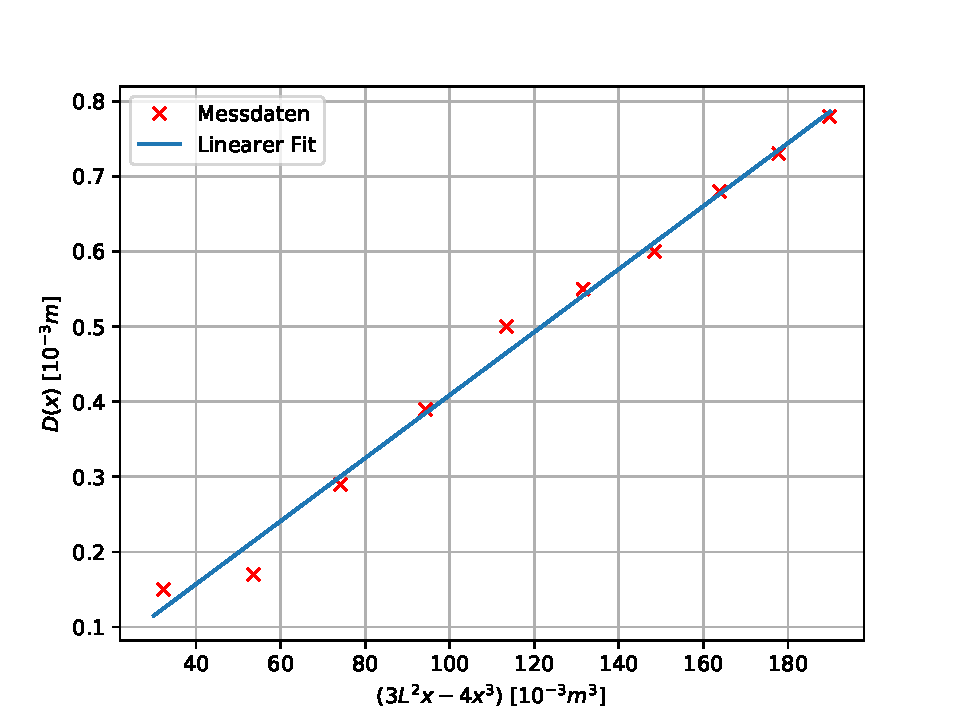
\includegraphics[width=0.9\linewidth]{beidseitig_rechts.pdf}
   \caption{Lineare Regression: Runder Stab, beidseitig aufgelegt, rechte Seite}
   \label{fig:beidseitig_rechts}
   \end{figure}
   
\begin{figure}[h!]
   \centering
   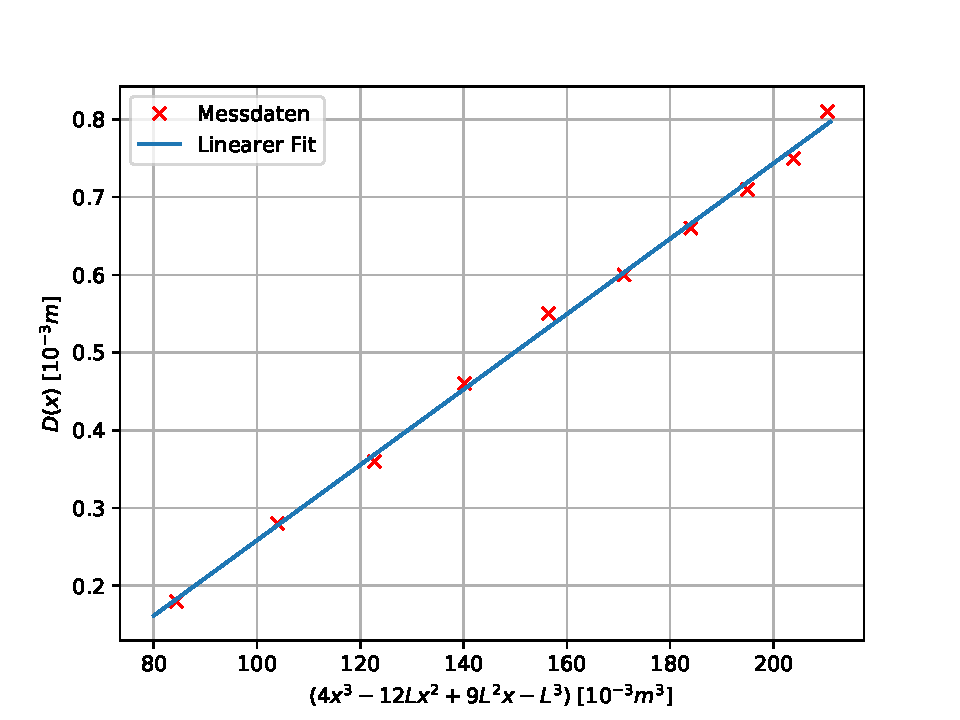
\includegraphics[width=0.9\linewidth]{beidseitig_links.pdf}
   \caption{Lineare Regression: Runder Stab, beidseitig aufgelegt, linke Seite}
   \label{fig:beidseitig_links}
   \end{figure}
   
Bei der beidseitigen Auflage werden jeweils die Elastizitätsmodule der linken und rechten Hälfte des Stabes berechnet.
Dafür werden die folgenden Hilfsfunktionen \cite[5,6]{anleitung103} verwendet:
\begin{equation*}
\begin{aligned}
\symup{Rechts}: 0 \leq x \leq \frac{L_{\text{r}}}{2}&: 3L_{\text{r}}^2x - 4x^3 \\
\symup{Links}: \frac{L_{\text{r}}}{2} \leq x \leq L_{\text{r}}&: 4x^3 - 2L_{\text{r}}x^2 + 9L_{\text{r}}^2x - L_{\text{r}}^3
\end{aligned}
\end{equation*}

Die Durchbiegungen $D(x)$ der jeweiligen Seite werden gegen die entsprechende Hilfsfunktion aufgetragen. Die Ausgleichsrechnung erfolgt über Matplotlib.
Es ergeben sich folgende Werte für die Steigungen und die Y-Achsenabschnitte:
\begin{equation*}
\begin{aligned}
a_{\text{br}} &= (0{,}0042 \pm 0{,}0001)\, \symup{\frac{1}{m^2}} \\
b_{\text{br}} &= (-0{,}01 \pm 0{,}02)\cdot 10^{-3} \, \symup{m} \\
\\
a_{\text{bl}} &= (0{,}005 \pm 0{,}008\cdot10^{-2})\, \symup{\frac{1}{m^2}} \\
b_{\text{bl}} &= (-0{,}23 \pm 0{,}01)\cdot 10^{-3} \, \symup{m}
\end{aligned}
\end{equation*}
Nun werden die beiden Gleichungen \eqref{eqn:e_beidseitig} nach $E$ umgestellt. Dadurch ergibt sich:
\begin{equation*}
E_{\text{br/bl}} = \frac{m_2\cdot g}{48\cdot I_{\text{r}} \cdot a_{\text{br/bl}}}.
\end{equation*}

Der zugehörige Fehler kann aus der Gauß'schen Fehlerfortpflanzung erhalten werden:
\begin{equation*}
 \begin{aligned}
 \Delta E_{\text{br/bl}} &= \sqrt{\biggl(\frac{\partial E_{\text{br/bl}}}{\partial I_{\text{r}}}\biggr)^2\cdot (\Delta I_{\text{r}})^2 + \biggl(\frac{\partial E_{\text{br/bl}}}{\partial a_{\text{br/bl}}}\biggr)^2\cdot (\Delta a_{\text{br/bl}})^2} \\
 \iff \Delta E_{\text{br/bl}} &= \sqrt{\biggl(\frac{m_2\cdot g}{48\cdot I_{\text{r}}^2 \cdot a_{\text{br/bl}}}\biggr)^2 \cdot (\Delta I_{\text{r}})^2 + \biggl(\frac{m_2\cdot g}{48\cdot I \cdot a_{\text{br/bl}}^2}\biggr)^2 \cdot (\Delta a_{\text{br/bl}})^2}.
 \end{aligned}
 \end{equation*}
Hiermit lauten die Elastizitätsmodule der beiden Seiten:
\begin{equation*}
\begin{aligned}
E_{\text{br}} &= (7{,}40 \pm 0{,}18)\cdot 10^9 \, \symup{\frac{N}{m^2}} \\
E_{\text{bl}} &= (6{,}22 \pm 0{,}17)\cdot 10^9 \, \symup{\frac{N}{m^2}}.
\end{aligned}
\end{equation*}
